
%(BEGIN_QUESTION)
% Copyright 2013, Tony R. Kuphaldt, released under the Creative Commons Attribution License (v 1.0)
% This means you may do almost anything with this work of mine, so long as you give me proper credit

This PLC-based lamp control system has a problem -- the ``ice-cube'' relay contacts fail prematurely after only a few months of service, necessitating periodic replacement of that relay.  Close inspection of the failed relay units reveals darkening and pitting of the metal contact faces:

$$\includegraphics[width=15.5cm]{i03358x01.eps}$$

First, describe a test (using a multimeter) to determine what is causing this relay to prematurely fail.  Be sure to identify not only where you would connect the meter in this circuit, but also how you would interpret the meter's reading to confirm the cause of the problem.

\vskip 10pt

Next, propose a practical solution for this problem.  If your solution requires any alteration of the circuit, be sure to explain in detail the changes to be made.

\underbar{file i03358}
%(END_QUESTION)





%(BEGIN_ANSWER)

I recommend half-credit for test and explanation, and half-credit for a practical solution to the problem:

\vskip 10pt

Relay contacts will prematurely fail if their maximum voltage and/or current contact ratings are exceeded.  Thus, an appropriate test would be a voltage measurement across the relay contacts when off (comparing this reading against the contacts' voltage rating) to see if that rating is being exceeded.  Another appropriate test would be a measurement of current through the contacts to see if the contacts' current rating is being exceeded.
 
\vskip 10pt

Irrelevant tests include anything to do specifically with the PLC, the input switches, the commutating diode, or the relay's coil.  The test must focus on either voltage or current through the relay {\it contacts} in order to receive credit for this half of the question.

\vskip 20pt

Practical solutions include replacing the interposing relay with a unit having higher contact ratings, paralleling the two sets of NO contacts on this relay for increased current capacity (if the test was for excessive current), reducing power requirements at the load, etc.  If the student's solution requires altering the circuit and their explalantion is insufficiently detailed, deduct 2 points.

%(END_ANSWER)





%(BEGIN_NOTES)


%(END_NOTES)


